\documentclass[
11pt,%
tightenlines,%
twoside,%
onecolumn,%
nofloats,%
nobibnotes,%
nofootinbib,%
superscriptaddress,%
noshowpacs,%
centertags]%
{revtex4}
\usepackage{ljm}
\usepackage{listings}

\lstset{
language=C++,
basewidth=0.5em,
xleftmargin=45pt,
xrightmargin=45pt,
basicstyle=\small\ttfamily,
keywordstyle=\bfseries\underbar,
numbers=left,
numberstyle=\tiny,
stepnumber=1,
numbersep=10pt,
showspaces=false,
showstringspaces=false,
showtabs=false,
frame=trBL,
tabsize=2,
captionpos=t,
breaklines=true,
breakatwhitespace=false,
escapeinside={\%*}{*)}
}

\begin{document}

\titlerunning{dataflow processor emulator}
\authorrunning{Kuznetsova and Rybakov}

\title{Features of Dataflow Processor Emulator Implementing}

\author{\firstname{E.~A.}~\surname{Kuznetsova}}
\email[E-mail: ]{mrallis@jscc.com}
\affiliation{Joint Supercomputer Center of the Russian Academy of Sciences -- branch of Scientific Research Institute of System Analysis of the Russian Academy of Sciences, Leninsky prospect 32a, Moscow, 119334, Russia}

\author{\firstname{A.~A.}~\surname{Rybakov}}
\email[E-mail: ]{rybakov.aax@gmail.com}
\affiliation{Joint Supercomputer Center of the Russian Academy of Sciences -- branch of Scientific Research Institute of System Analysis of the Russian Academy of Sciences, Leninsky prospect 32a, Moscow, 119334, Russia}

\firstcollaboration{(Submitted by S.~S.~Submitter)}

\received{May 01, 2020}

\begin{abstract}
Развитие архитектур потоковых процессоров является перспективным направлением повышения производительности вычислительных систем.
Потоковые процессоры обладают рядом преимуществ по сравнению с процессорами архитектуры фон Неймана.
Данные преимущества выражены в явном параллелизме вычислений, так как в представлении программ для потокового процессора последовательность выполнения инструкций ограничена исключительно фактом готовности их входных данных.
Концепция использования токенов в качестве носителей данных для инструкций позволяет снять множество проблем, связанных с конфликтами по данным, и позволяет упростить логику программы.
Важнейшим элементом реализации логики потокового процессора является ассоциативная память токенов, которая должна обеспечивать хранение и быстрый поиск готовых данных для инструкций, которые могут быть отправлены на выполнение.
В данной статье рассматривается функционал ассоциативной памяти токенов и логика ее работы на примере простого потокового графа.
\end{abstract}

\subclass{68N20,68R10} % Enter 2010 Mathematics Subject Classification.

\keywords{Dataflow processor emulator, dataflow graph, token, token state, associative memory, control flow graph, def-use graph.}

\maketitle

\section{Introduction}

Введение про архитектуру потокового процессора.

\section{Эмуляция работы процессора с архитектурой фон Неймана}

Одним из основных принципов архитектуры фон Неймана является принцип последовательного программного управления.
Согласно ему исполняемый код программы хранится в памяти, и его инструкции могут быть выполнены процессором последовательно, одна за другой.
Адрес следующей инструкции, подаваемой процессору на выполнение, хранится в специальном регистре, называемом instruction pointer, по умолчанию он всегда сдвигается на следующую инструкцию в памяти.
Данный адрес может быть принудительно изменен специальными инструкциями перехода, в этом случае можно говорить о передаче управления на другую часть программы.

Введем понятие линейного участка (или базового блока программы).
Линейным участком будем называть последовательность инструкций со следующими двумя свойствами.
Во-первых, управление может быть передано только на первую инструкцию данного участка (иными словами у линейного участка есть только один вход, которым является первая инструкция участка).
Во-вторых, если управление передано на линейный участок, то обязательно должны быть выполнены все инструкции данного участка (то есть внутри линейного участка не может быть инструкций перехода, инструкция перехода может находиться только в конце линейного участка).
Иногда вместо линейных участков удобно рассматривать так называемые квазилинейные участки, внутри которых может находиться произвольное количество инструкций переходов на другие линейные участки.
Мы не будем касаться квазилинейных участков, так как любой такой участок можно разбить на последовательность обычных линейных участков.

Важным понятием, широко используемым в теории оптимизирующих компиляторов, является граф потока управления \cite{Muchnick}.
Графом потока управления называют ориентированный граф, узлами которого являются линейные участки программы, а дугами показана передача управления между ними.
Граф потока управления является удобной и наглядной структурой для описания поведения программы и используется оптимизирующими компиляторами для осуществления глобальных оптимизаций программы, то есть оптимизаций, выходящих за рамки линейных участков.

Рассмотрим логику устройства промежуточного представления программы внутри одного линейного участка.
Для этого рассмотрим простой пример нахождения корней квадратного уравнения.
Для записи примеров и псевдокода будем использовать листинги на языке программирования С.
Итак, пусть у нас есть линейный участок (блок кода программы), на входе в который мы имеем переменные $a$, $b$, $c$, содержащие коэффициенты квадратного уравнения $ax^2 + bx + c = 0$.
Требуется на выходе из линейного участка получить значения корней, которые вычисляются по формулам $x_{1,2} = (-b \pm \sqrt{b^2 - 4ac})/(2a)$.

\begin{lstlisting}[caption={Текст блока кода по вычислению корней квадратного уравнения.},label={lst:square_equation_1}]
{
    float t = sqrt(b * b - 4.0 * a * c);
    
    x1 = (-b + t) / (2.0 * a);
    x2 = (-b - t) / (2.0 * a);
}
\end{lstlisting}

\

В листинге~\ref{lst:square_equation_1} линейный участок специально выделен в фигурные скобки и объявлена временная переменная $t$, чтобы было понятно, что за пределами линейного участка данная переменная не используется.
Для удобства будем считать, что процессор, для которого будет создаваться исполняемый код, поддерживает инструкцию вычисления квадратного корня.
Таким образом, в приведенном листинге будут фигурировать следующие инструкции по работе с вещественными числами: MUL -- умножение двух чисел, SUB -- разность двух чисел, SQRT -- квадратный корень числа, NEG -- унарный минус, ADD -- сложение двух чисел, DIV -- частное двух чисел.

\begin{figure}[h]
\setcaptionmargin{5mm}
%\onelinecaptionsfalse % if the caption is multiline
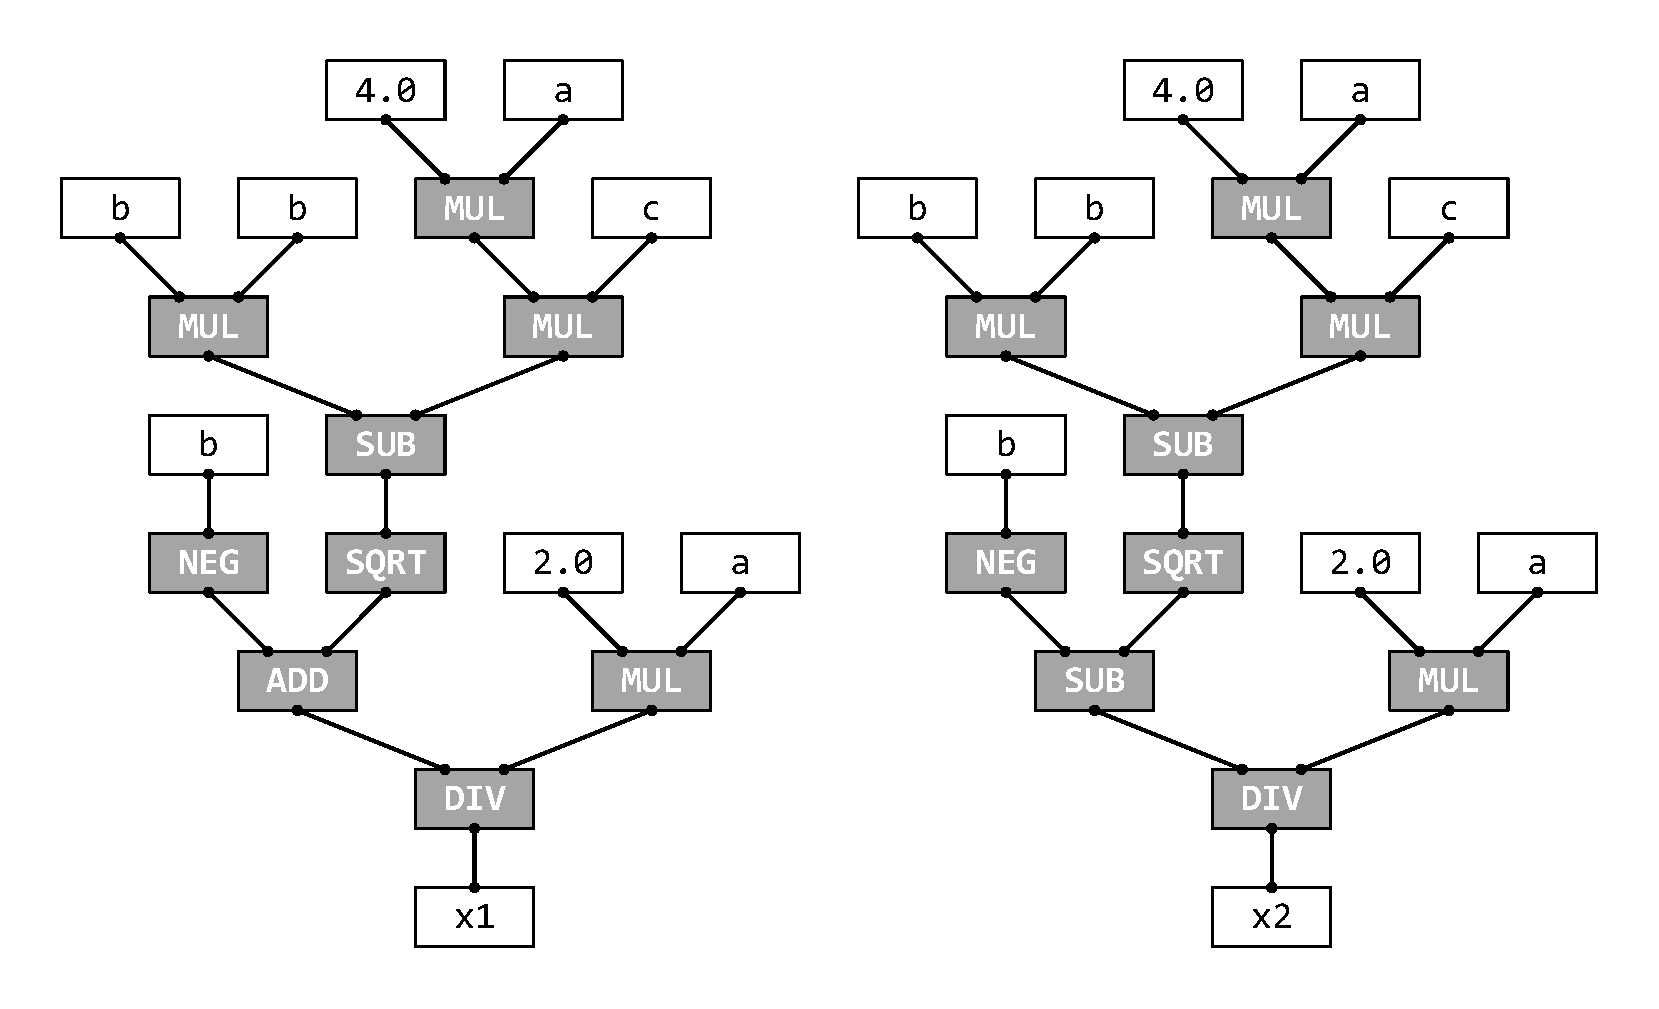
\includegraphics[width=0.95\textwidth]{pics/square_equation_calculation_tree.pdf}
\captionstyle{normal}\caption{Дерево вычисления выражений корней квадратного уравнения.}\label{fig:square_equation_calculation_tree}
\end{figure}

На рисунке~\ref{fig:square_equation_calculation_tree} показаны два дерева вычисления выражений $x_1$ и $x_2$.
Компилятор, конечно упростит данные вычислений с помощью сбора общих подвыражений, и финальная версия представления линейного участка будет близка к следующему графу зависимостей, приведенному на рисунке~\ref{fig:def_use}.

\begin{figure}[h]
\setcaptionmargin{5mm}
\onelinecaptionsfalse % if the caption is multiline
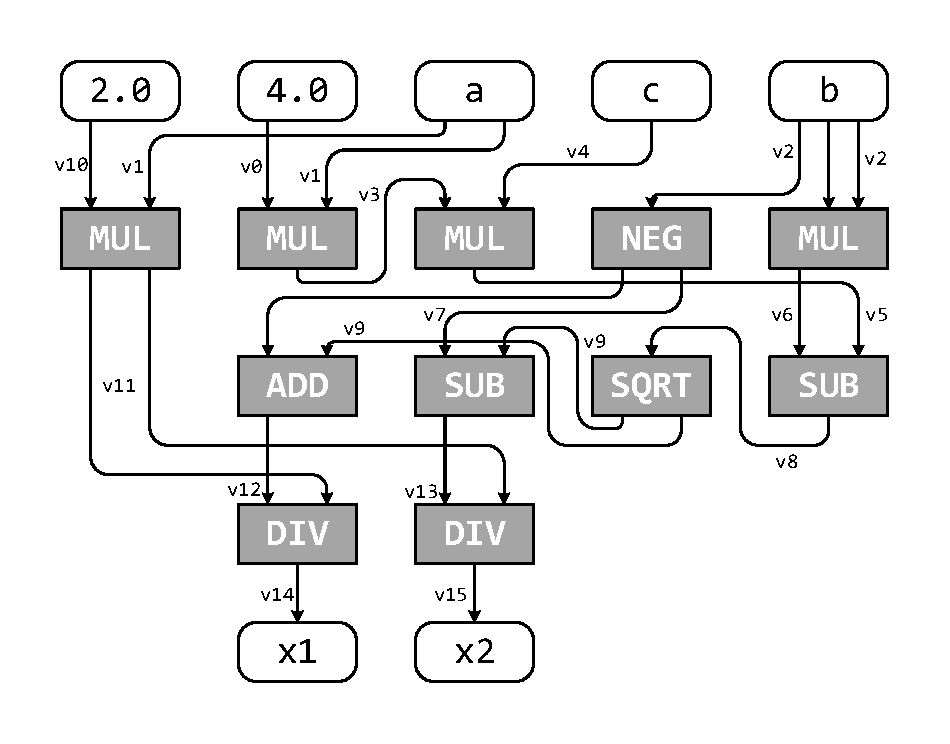
\includegraphics[width=0.60\textwidth]{pics/def_use.pdf}
\captionstyle{normal}\caption{Граф зависимостей линейного участка при вычислении выражений\\ корней квадратного уравнения.}\label{fig:def_use}
\end{figure}

Узлами данного ориентированного графа являются отдельные операции (показаны темными прямоугольниками), а дугами -- def-use зависимости между операциями по данным (команда $B$ зависит по данным от команды $A$, если потребляет данные, вырабатываемые командой $A$).
Кроме зависимостей по данным могут быть и другие зависимости между операциями (зависимости по управлению, антизависимости), однако в нашем простом примере данные зависимости отсутствуют.

Для формирования результирующего исполняемого кода не достаточно наличия def-use графа.
Необходимо выстроить все команды, входящие в def-use граф, в единую последовательность, которая в дальнейшем будет записана в последовательный участок памяти.
При этом при выстраивании последовательности команд необходимо соблюдать требование, что если команда $B$ зависит от команды $A$ по данным, то в финальной последовательности она должна стоять позже команды $A$.
Данный процесс называется планированием кода \cite{Aho}.
В результате выполнения планирования кода для рассматриваемого примера получим псевдокод вычисления корней квадратного уравнения примерно в следующем виде, показанном в листинге~\ref{lst:square_equation_2}.

\begin{lstlisting}[caption={Псевдокод вычисления корней квадратного уравнения.},label={lst:square_equation_2}]
MOV 4.0       ->  v0
MOV   a       ->  v1
MOV   b       ->  v2
MUL  v0,  v1  ->  v3
MOV   c       ->  v4
MUL  v3,  v4  ->  v5
MUL  v2,  v2  ->  v6
NEG  v2       ->  v7
SUB  v6,  v5  ->  v8
SQRT v8       ->  v9
MOV 2.0       -> v10
MUL v10,  v1  -> v11
ADD  v7,  v9  -> v12
SUB  v7,  v9  -> v13
DIV v12, v11  -> v14
DIV v13, v11  -> v15
MOV v14       ->  x1
MOV v15       ->  x2
\end{lstlisting}

\

В листинге~\ref{lst:square_equation_2} все инструкции кроме операций пересылок оперируют с виртуальными регистрами (v0-v15).
В данном записи важен порядок следования команд.
В любой момент времени после выполнения любой инструкции мы можем говорить об некотором состоянии процессора, которое характеризуется содержимым памяти, а также всех используемых регистров.

Основной частью эмулятора процессора является реализация семантики инструкций, выполняемых процессором.
То есть каждая инструкция рассматривается как функция, которая переводит вычислительную машину из одного состояния в другое.

\section{Эмуляция работы потокового процессора}

В отличие от процессоров с архитектурой фон Неймана, в потоковых процессорах отсутствует полная упорядоченность выполнения команд.
То есть если какие-то две инструкции могут быть выполнены параллельно (это позволяет сделать отсутствие зависимостей между ними), то порядок их выполнения не определен.
Будем рассматривать все тот же пример одного линейного участка, внутри которого происходит вычисление корней квадратного уравнения.
Программа для потокового процессора представляет собой граф, очень похожий на def-use граф, представленный на рисунке~\ref{fig:def_use}.
Потоковый граф, который представляет собой программу для потокового процессора, также является ориентированным.
Узлами данного графа также являются инструкции, выполняемые процессором, однако ребра носят принципиально другой смысл.
Если в случае def-use графа ребро являлось фиксацией факта зависимости между двумя операциями (с указанием, по какой переменной, по какому ресурсу), то в потоковом графе ребро является носителем уникальной единицы данных, называемой токеном.
Итак, токен -- это структура данных, хранящая информацию о передаваемых данных, а также о точке назначения этих данных (идентификатор потребляющий эти данные инструкции, а также номер аргумента, которым эти данные являются для инструкции).
Кроме того, токен содержит дополнительные сведения (состояние токена), позволяющие различать инструкции, относящиеся к разным вызовам функции или к разным итерациям цикла, однако для данного примера это не является важным, поэтому описание состояния токена опустим.

\begin{figure}[h]
\setcaptionmargin{5mm}
\onelinecaptionsfalse % if the caption is multiline
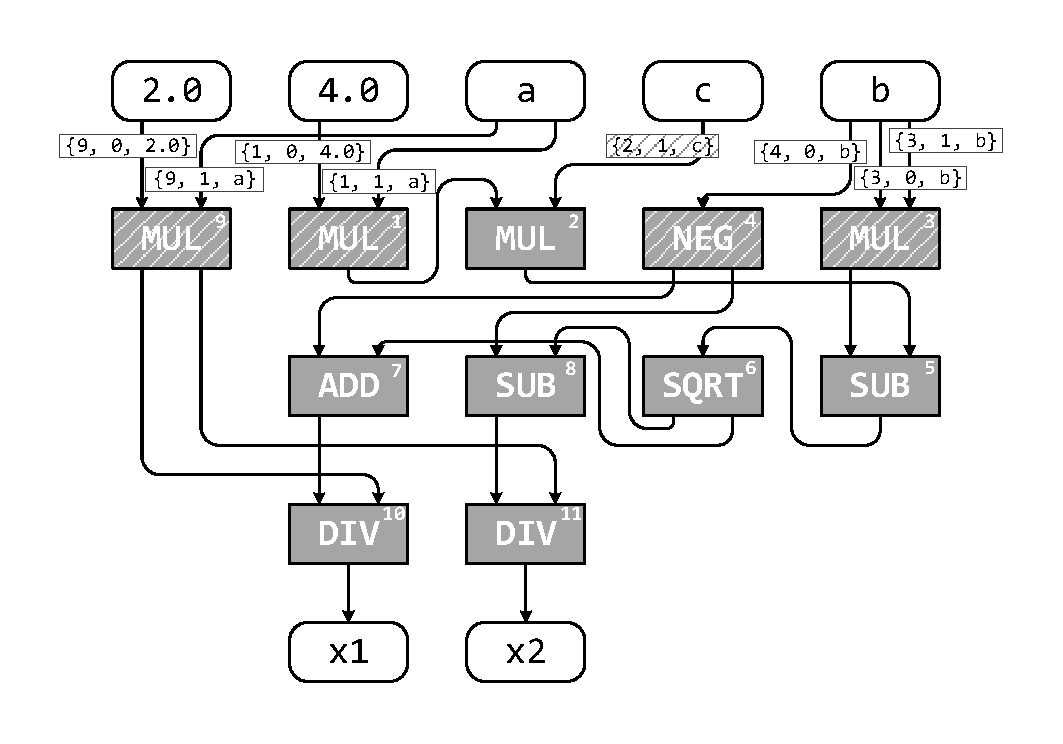
\includegraphics[width=0.80\textwidth]{pics/dataflow.pdf}
\captionstyle{normal}\caption{Потоковый граф линейного участка при вычислении выражений\\ корней квадратного уравнения.}\label{fig:dataflow}
\end{figure}

На рисунке~\ref{fig:dataflow} показан потоковый граф в начальный момент времени, когда ни одна из инструкций еще не была выполнена.
На данном рисунке на ребрах графа можно видеть те токены, которые готовы и поданы на соответствующие инструкции.
Например, для инструкции 9 MUL готовы два токена: $\{9, 0, 2.0\}$ (9 -- номер инструкции, 0 -- номер аргумента, 2.0 -- вещественное число), $\{9, 1, a\}$ (9 -- номер инструкции, 1 -- номер аргумента, $a$ -- вещественное число).
То есть оба аргумента для инструкции 9 MUL готовы и инструкция может быть выполнена.
После выполнения токены, содержащие аргументы, удаляются, а по выходным дугам к инструкциям 10 DIV и 11 DIV будут направлены токены, содержащие результат инструкции 9 MUL.

Если рассмотреть другую инструкцию 2 MUL, то можно заметить, что для нее готов только второй аргумент (токен $\{2, 1, c\}$).
Первый аргумент будет сформирован только после выполнения инструкции 1 MUL.

Таким образом все инструкции в представленном графе будут обработаны, пока требуемые значения не будут получены в токенах на выходных дугах из инструкций 10 DIV и 11 DIV.

Реализация семантики инструкций в эмуляторе потокового процессора ничем не отличается от такого же функционала в эмуляторе традиционного процессора.

Центральным функциональным элементом для обеспечения работоспособности потокового процессора является так называемая ассоциативная память токенов, реализация которой является назначением данной статьи.

Ассоциативная память токенов представляет собой хранилище токенов, которые в данный момент созданы и находятся на выполнении в программе.
При этом, если оказывается, что в ассоциативной памяти находятся все необходимые аргументы для какой-либо команды, они сразу же удаляются из ассоциативной памяти и отправляются на исполнение в команду.
Таким образом, в любой момент времени в ассоциативной памяти находятся только те аргументы, которые ждут недостающих аргументов для некоторых инструкций.
То есть в условно первый момент времени, представленный на рисунке~\ref{fig:dataflow}, в ассоциативной памяти токенов находится только один токен $\{2, 1, c\}$, ждущий свою пару, тогда как команды 9 MUL, 1 MUL, 4 NEG, 3 MUL уже готовы к исполнению и находятся в буфере команд вместе с наборами своих аргументов.
На рисунке~\ref{fig:dataflow} заштрихован токен, находящийся в ассоциативной памяти, а также команды, готовые к выполнению.

\begin{figure}[h]
\setcaptionmargin{5mm}
\onelinecaptionsfalse % if the caption is multiline
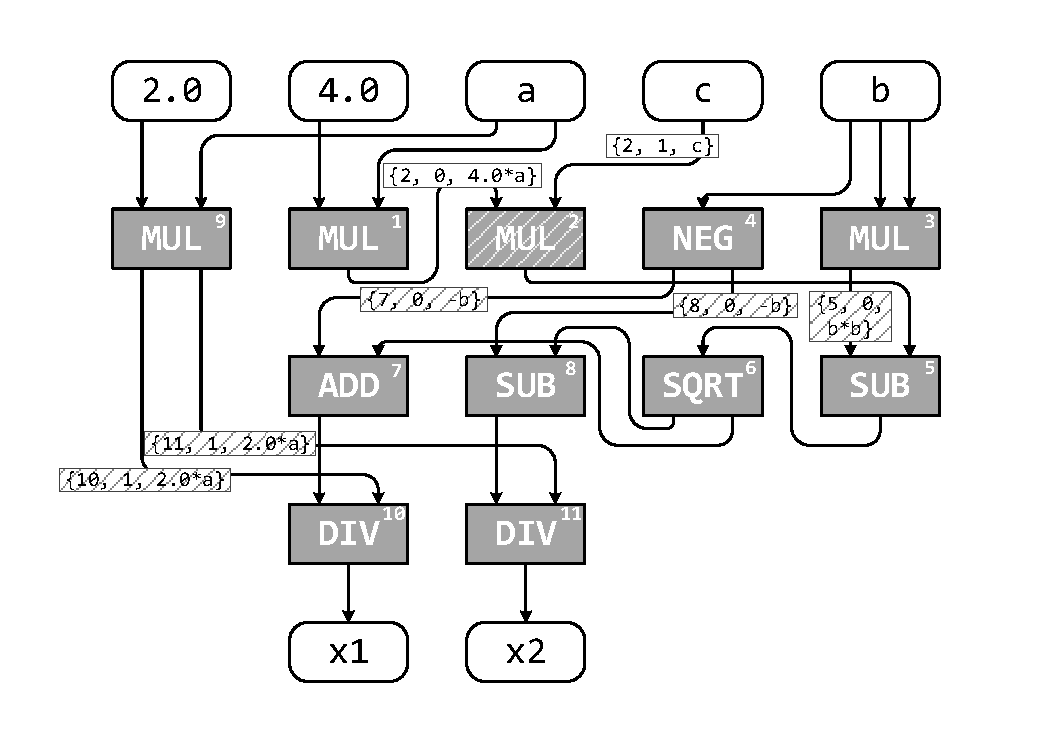
\includegraphics[width=0.80\textwidth]{pics/dataflow2.pdf}
\captionstyle{normal}\caption{Потоковый граф линейного участка при вычислении выражений корней квадратного уравнения перед выполнением инструкции 2 MUL.}\label{fig:dataflow2}
\end{figure}

После выполнения инструкций 9 MUL, 1 MUL, 4 NEG и 3 MUL единственной инструкцией, готовой к исполнению, является 2 MUL.
Состояние машины перед выполнением этой инструкции показано на рисунке~\ref{fig:dataflow2}.
На данном рисунке видна готовая к выполнению инструкция 2 MUL, а также несколько токенов, попавших в ассоциативную память.
Дальнейшее выполнение программы происходит аналогично и в конце мы приходим к формированию двух токенов по выходным дугам операций 10 DIV и 11 DIV, которые далее будут направлены к своим инструкциям-потребителям.

\begin{lstlisting}[caption={Реализация логики ассоциативной памяти токенов.},label={lst:assoc}]
set_token({CId, E, _} = T, Args, D) when (Args > 1) ->
	FullEntries = lists:seq(0, Args - 1, 1),
	ET = {E, T},
	case dict:find(CId, D) of
		error ->
			dict:append(CId, ET, D);
		{ok, Vs} ->
			{Es, Ts} = lists:unzip(lists:sort(Vs ++ [ET])),
			case Es of
				FullEntries ->
					{Ts, dict:erase(CId, D)};
				_ ->
					dict:append(CId, ET, D)
			end
	end.
\end{lstlisting}

\

В листинге~\ref{lst:assoc} приведена компактная реализация логики ассоциативной памяти токенов на языке Erlang \cite{Armstrong}.
Вся логика реализуется с помощью одной функции $set\_token$ с тремя аргументами: $T$ -- добавляемый токен (который состоит из идентификатора инструкции $CId$, номера аргумента $E$, и данных), $Args$ -- количество аргументов у инструкции, для которой добавляется токен, $D$ -- словарь, с помощью которого реализована ассоциативная память токенов.
Логика функции сводится к следующему: извлечь из словаря, все токены, ассоциированные с ключом $CId$, и проверить, закрывают ли они все аргументы рассматриваемой инструкции (то есть номера аргументов формируют последовательность $[0, 1, .. Args - 1]$.
Если добавляемый токен представляет собой последний недостающий аргумент рассматриваемой инструкции, то требуется извлечь из словаря все токены и вернуть их в виде списка на исполнение инструкции (строка 11).
В противном случае токен следует добавить в словарь, привязав к ключу $CId$ (строки 6 и 13).

Заметим, что приведена наиболее упрощенная реализация.
В ней не рассматривается возможность использования состояния токена для идентификации инструкций из разных вызовов функции или с разных итераций цикла (для полноты картины в качестве ключа словаря наряду с идентификатором инструкции $CId$ следует использовать также состояние токена).
Также в приведенной реализации не рассматривается обработка исключительных ситуаций.
Например, последовательное добавление в ассоциативную память двух токенов, представляющих один и тот же аргумент одной и той же инструкции, должно вызывать ошибку.
Однако, несмотря на неполноту реализации, приведенная логика позволяет обеспечить функционал ассоциативной памяти токенов, необходимый для выполнения программы для потокового процессора.

\section{Conclusion}

В статье рассмотрены отличия в реализации выполнения исполняемой программы, предназначенной для процессара с архитектурой фон Неймана и для потокового процессора.
Показаны отличия def-use графа и потокового графа, которые отражают логику программы в рамках линейного участка.
Рассмотрен необходимый элемент реализации эмулятора потокового процессора -- ассоциативная память токенов, с помощью которой можно хранить и быстро находить готовые данные для команд, которые могут быть переданы на исполнение.
Приведена компактная реализация ассоциативной памяти токенов для инструкций с произвольным количеством итераций.
Данная реализация может быть расширена для произвольной программы для потокового процессора, в том числе в которой используются циклы и вызовы функций (в том числе рекурсивные).
Данный подход к организации ассоциативной памяти токенов используется в реализации эмулятора векторного потокового процессора, архитектура которого разрабатывается в МСЦ РАН.

\begin{acknowledgments}
The work has been done at the JSCC RAS as part of the state assignment for the topic ... The supercomputer MVS-10P, located at the JSCC RAS, was used for calculations during the research.
\end{acknowledgments}

\begin{thebibliography}{99}

\bibitem{Muchnick}
\refitem{book}
S.~S.~Muchnick, {\it ``Advanced Compiler Design \& Implementation."}, Academic Press (1997).

\bibitem{Aho}
\refitem{book}
A.~V.~Aho, M.~S.~Lam, R.~Sethi, J.~D.~Ullman, {\it ``Compilers. Principles, Techniques, \& Tools."}, Addison-Wesley (2007).

\bibitem{Armstrong}
\refitem{book}
J.~Armstrong, {\it ``Programming Erlang. Software for a Concurrent World."}, Pragmatic Programmers (2013).

\end{thebibliography}

\end{document}
